\chapter{Modelling} \label{cha:chapter-3}

\section{Logistic Regression}

\section{Results}

Data was split into train and test sets with proportions 0.7 and 0.3 respectively. Bad rate was maintained in each data set at 17\%. The woe values from tables  (\ref{woe_1}) \& (\ref{woe_2}) were applied. Once split the train data was passed through a glm model with logit link, for this the statsmodel package was used \cite{statsmodels}. Three models were run and compared  (\ref{glm_out}).  

\begin{figure}
\begin{center}
\begin{tabular}{lclc}
\toprule
\textbf{Dep. Variable:}  &       BAD        & \textbf{  No. Observations:  } &     3522    \\
\textbf{Model:}          &       GLM        & \textbf{  Df Residuals:      } &     3510    \\
\textbf{Model Family:}   &     Binomial     & \textbf{  Df Model:          } &       11    \\
\textbf{Link Function:}  &      logit       & \textbf{  Scale:             } &    1.0000   \\
\textbf{Method:}         &       IRLS       & \textbf{  Log-Likelihood:    } &   -1236.8   \\
\textbf{Date:}           & Sat, 15 Aug 2020 & \textbf{  Deviance:          } &    2473.6   \\
\textbf{Time:}           &     13:16:04     & \textbf{  Pearson chi2:      } &  3.55e+03   \\
\textbf{No. Iterations:} &        6         & \textbf{                     } &             \\
\bottomrule
\end{tabular}
\begin{tabular}{lcccccc}
                      & \textbf{coef} & \textbf{std err} & \textbf{z} & \textbf{P$> |$z$|$} & \textbf{[0.025} & \textbf{0.975]}  \\
\midrule
\textbf{const}        &      -1.6002  &        0.054     &   -29.683  &         0.000        &       -1.706    &       -1.495     \\
\textbf{CLNO\_woe}    &       0.8862  &        0.154     &     5.755  &         0.000        &        0.584    &        1.188     \\
\textbf{REASON\_woe}  &      -0.1580  &        0.455     &    -0.347  &         0.729        &       -1.051    &        0.735     \\
\textbf{VALUE\_woe}   &       0.8818  &        0.159     &     5.558  &         0.000        &        0.571    &        1.193     \\
\textbf{YOJ\_woe}     &       1.1226  &        0.214     &     5.238  &         0.000        &        0.703    &        1.543     \\
\textbf{DELINQ\_woe}  &       1.0389  &        0.072     &    14.443  &         0.000        &        0.898    &        1.180     \\
\textbf{LOAN\_woe}    &       0.7584  &        0.115     &     6.581  &         0.000        &        0.533    &        0.984     \\
\textbf{DEROG\_woe}   &       0.8037  &        0.100     &     8.062  &         0.000        &        0.608    &        0.999     \\
\textbf{CLAGE\_woe}   &       0.8006  &        0.102     &     7.861  &         0.000        &        0.601    &        1.000     \\
\textbf{NINQ\_woe}    &       1.0246  &        0.139     &     7.397  &         0.000        &        0.753    &        1.296     \\
\textbf{JOB\_woe}     &       0.7379  &        0.155     &     4.764  &         0.000        &        0.434    &        1.041     \\
\textbf{MORTDUE\_woe} &       0.0044  &        0.234     &     0.019  &         0.985        &       -0.455    &        0.464     \\
\bottomrule
\end{tabular}
\caption{Generalized Linear Model Regression Results \label{glm_out}}
\end{center}
\end{figure}

\begin{figure}
\begin{center}
\renewcommand{\arraystretch}{1.25}
\begin{tabular}{lccc}
\toprule
Model & AIC & KS & GINI \\
Model 1 (Default) & 2497.64 & 0.4616 & 0.5985 \\
Model 2 (REASON and MORTDUE dropped) & 2493.76 & 0.4584 & 0.5985 \\
Model 3 (Log transformations) & 2504.0873 & 0.4753 & 0.5993 \\
\bottomrule
\end{tabular}
\caption{Performance Evaluation Results On Test \label{perf_eval}}
\end{center}
\end{figure}

\begin{figure}[!ht]
	\centering
	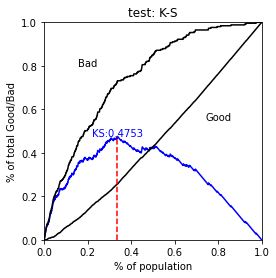
\includegraphics[scale=0.90]{figs/ks_plot.png}
	\caption{KS Plot \label{ks_plot}}
\end{figure}

\begin{figure}[!ht]
	\centering
	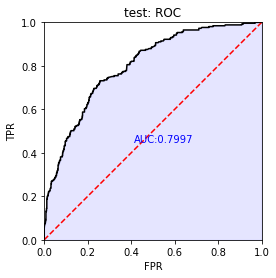
\includegraphics[scale=0.90]{figs/roc_plot.png}
	\caption{ROC Plot \label{roc_plot}}
\end{figure}

\begin{landscape}
\begin{figure}[!ht]
\begin{center}
	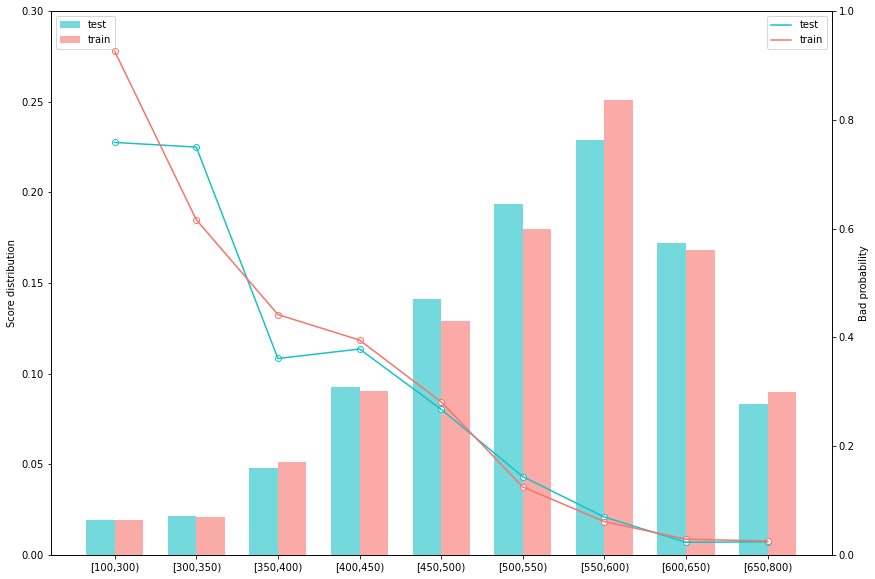
\includegraphics[scale=0.75]{figs/scorecard_plot.png}
	\caption{Scorecard Plot \label{scorecard_plot}}
\end{center}
\end{figure}
\end{landscape}

%\section{Ridge Regression}
%The Ridge Regression method or also know as Tikhonov regularization originally began being developed by Andre Tikhonov in Russia and published in the book "Solutions of ill-posed problems". During around the same time as Andre. two American statiticians, Arthur Hoerl and Robert Kennardcan, released the paper "Ridge Regression: Biased Estimation for Nonorthogonal Problems" in 1970. Ridge regression can be useful to apply when there is a large number of predictors which all seem to have a small effect on the response variable of interest. Applying ridge regression to the data produces a shrinking effect on the predictors and some can effectively reach zero but the method cannot reduce the estimates to exactly zero. As the coefficients shrink this does produce bias but also reduces the variance of the estimates.\cite{hoerl1970ridge}\cite{marquardt1975ridge}\\
%
%\paragraph{\textbf{Ridge Estimate}}Assume $\bm{X}$ is a $n$ by $p$ matrix and $\bm{Y}$ is an $n$ vector. The ridge regression estimator is given by:
%
%\begin{equation}
%\hat{\bm{\beta}}_{ridge} = (\bm{X^{'} X} + \lambda \bm{I}_p)^{-1} \bm{X^{'} Y}
%\end{equation}
%
%or can be seen as the values minimizing\cite{james2013introduction}:
%
%\begin{equation}
%\sum\limits_{i=1}^n\left(y_i-\beta_0-\sum\limits_{j=1}^p\beta_j x_{ij}\right)^2 + \lambda\sum\limits_{j=1}^p\beta_j^2=RSS + \lambda\sum\limits_{j=1}^p\beta_j^2
%\end{equation}
%
%Or similarly can be seen as:
%
%\begin{equation}
%\hat{\bm{\beta}} = arg \min\limits_{\bm{\beta}} \sum\limits_{i=1}^n \left(y_i-\sum\limits_{j=1}^p x_{ij}\beta_j \right)^2 \text{ subject to } \sum\limits_{j=1}^p \beta_j^2 < t
%\end{equation}
%
%where t is the tuning parameter.\\
%
%$\sum\limits_{j=1}^p \beta_j^2 < t$ is called the shrinkage penalty and can become very small when $\beta_1 ... \beta_p$ are close to zero. This shrinking penalty is not applied to our intercept as we only want to shrink the variables estimators. When our tuning parameter, $\lambda$, is set to zero, we are able to produce least squares estimates and for every possible value for $\lambda$ we will produce a different set of estimates for our predictors. Because of this it is important that the selection for the tuning parameter is as optimal as possible. Choosing the right value for the tuning parameter is also important to keep bias to a minimum while also reducing the variance of the estimates as much as possible.\cite{friedman2001elements} \\
%
%One way to select and appropriate value for $\lambda$ is through cross-validation. In order to do this we take a range of values for $\lambda$ and pick the value of $\lambda$ at which the cross-validation error is smallest.\\
%
%Although the ridge regression can be effective, the large problem if I was to use only this method would be that I am unable to reduce the amount of predictors used. Since the method is unable to exclude predictors and simply reduces redundant ones to very small values, the model will end up containing all 13 variables. There are many problems for this and sometimes is not ideal.\\
%
%\section{LASSO}
%LASSO(Least absolute shrinkage and selection operator) was first proposed by Robert Tibshirani\cite{tibshirani1996regression} in 1996. Introduced as an alternative for Ridge regression, The LASSO method is designed to minimize the residual sum of squares through an L1-norm. LASSO penalizes through an L1-norm (least absolute deviations) which minimizes the sum of the absolute differences. Sometimes this can result in reducing a coefficient to effectively zero. Providing what the method believes to be the most significant predictors. LASSO similar to ridge is a penalized regression method and produces bias in order to decrease the variance of the coefficients.
%\begin{defn}\cite{tibshirani1996regression}
%Suppose that we have data $(\bm{x}^i, y_i)$, $i=1,2,...,N$, where $\bm{x}^i = (x_{i1},...,x_{ip})^T$ are the predictor variables and $y_i$ are the responses. As in the usual regression set-up, we assume either that the observations and independent or that the $y_i$s are conditionally independent given the $x_{ij}$s. We assume that the $x_{ij}$ are standardized so that $\Sigma_i x_{ij}/N = 0$, $\Sigma_i x^2_{ij}/N = 1$.\\
%\\
%
%\paragraph{\textbf{LASSO Estimate}}
%The LASSO estimates can be found by minimizing this problem\cite{james2013introduction}:
%
%\begin{equation}
%\sum\limits_{i=1}^n\left(y_i-\beta_0-\sum\limits_{j=1}^p\beta_j x_{ij}\right)^2 + \lambda\sum\limits_{j=1}^p|\beta_j|=RSS + \lambda\sum\limits_{j=1}^p|\beta_j|
%\end{equation}
%
%Or similarly by letting $\bm{\hat{\beta}}=(\hat{\beta}_1,...,\hat{\beta}_p)^T$, the lasso estimate $(\hat{\alpha}, \hat{\beta})$ is defined by
%
%\begin{equation}
%(\hat{\alpha},\hat{\beta})=arg \min{\left\lbrace\sum\limits_{i=1}^N\left(y_i - \alpha - \sum\limits_j \beta_j x_{ij}\right)^2\right\rbrace} \qquad  \text{Subject to }\sum\limits_j |\beta_j| \leq t
%\end{equation}
%
%Where $t\geq0$ is a tuning parameter. $t$ controls the amount of shrinkage that is applied to the estimates.
%\end{defn}
%
%As you can see, Ridge and LASSO are fairly similar with the difference being in the shrinkage penalty. For Ridge we have $\beta_j^2$ and for LASSO we have $|\beta_j|$. Just like Ridge regression, LASSO has a shrinking effect on the predictors but with LASSO's shrinking penalty some estimates can be shrunk enough to be set to exactly zero effectively removing some variables. This produces a variable selection method, giving us a smaller model for interpretation. So as is with Ridge regression, it is important that we choose a suitable value for $\lambda$ and we can again use cross-validation to find that suitable value.\cite{friedman2001elements}
%
%\section{Elastic Net}
%The Elastic Net method is known to be a combination of both Ridge regression and Lasso, allowing the coefficients to be shrunk and in some cases set to zero. Introduced by Zou, Hui, and Trevor Hastie, It is considered, based on real world data and simulations, to out perform the LASSO method\cite{zou2005regularization}. One of the effects of the Elastic Net is that it causes grouping. Predictors which have strong correlations between each other are usually either left in or out together.\cite{zou2005regularization}\\
%\\
%In the paper by Hui and Hastie, they first define the Naive Elastic Net.
%\begin{defn}\cite{zou2005regularization}
%Suppose that the data set has $n$ observations with $p$ predictors. Let $\bm{y} = (y_1,..., y_n)^T$ be the response and $\bm{X} = (\bm{x}_1|...|\bm{x}_p)$ be the model matrix, where $\bm{x}_j = (x_{1j},..., x_{nj})^T, \quad j =1,...,p$, are the predictors. After a location and scale transformation, we can assume that the response is centred and the predictors are standardized,
%
%\begin{equation}
%\sum\limits_{i=1}^n y_i=0, \quad \sum\limits_{i=1}^n x_{ij}=0, \quad \text{and } \sum\limits_{i=1}^n x_{ij}^2=1, \qquad \text{for } j=1,2,...,p
%\end{equation}
%
%The naive elastic net estimate can be determined by minimizing
%
%\begin{equation}
%\hat{\bm{\beta}}= arg \min\limits_{\bm{\beta}} \left\lbrace \vert Y - \bm{X\beta} \vert^2 +\lambda_2\vert\bm{\beta}\vert^2 + \lambda_1\vert\bm{\beta}\vert_1 \right\rbrace
%\end{equation}
%
%where 
%
%\begin{equation}
%\vert\bm{\beta}\vert^2 = \sum\limits_{j=1}^p \beta_j^2 \text{ and } \vert\bm{\beta}\vert_1 = \sum\limits_{j=1}^p \vert\beta_j\vert 
%\end{equation}
%
%By letting $\alpha = \frac{\lambda_1}{\lambda_1 + \lambda_2}$, solving $\hat{\beta}$ can be seen as optimizing:\cite{Net}
%
%\begin{equation}
%\hat{\bm{\beta}} = arg \min\limits_{\bm{\beta}} \vert Y - \bm{X\beta} \vert^2, \text{ subject to } (1-\alpha)\vert\beta\vert_1 + \alpha\vert\beta\vert^2 \leq t \text{ for some t.}
%\end{equation}
%
%$(1-\alpha)\vert\beta\vert_1 + \alpha\vert\beta\vert^2$ is considered the elastic net penalty\cite{zou2005regularization}, which is a convex combination of the lasso and ridge penalty. Where letting $\alpha = 1$ causes a ridge penalty and $\alpha = 0$ allows a lasso penalty to be applied.
%\end{defn}
%
%Although the method still needs improvement. Using the naive elastic estimate brings a result similar to either a Ridge regression or a Lasso regression and does not produce a combination of both when applied. It produces an effect of shrinking the estimates twice as both the ridge and lasso methods produce shrinking. To solve this the elastic net estimate is provided. which is simply a rescaled estimate of the naive elastic estimate:
%
%\begin{equation}
%\hat{\bm{\beta}}\text{(elastic net)} = (1 + \lambda_2)\hat{\bm{\beta}}\text{(naive elastic net)}
%\end{equation}
%
%\section{Information Criterions}
%
%Once I have produced all three models from my methods I will need to select the one which fits my data the best. I have decided to use two information criterions, Akiake's\cite{hu2007akaike} and Bayesian's to select my final model.\\
%
%\begin{defn}\cite{posada2004model}
%The AIC for a given model is a function of its maximized likelihood (L) and the number of estimable parameters (K):
%
%\begin{equation}
%AIC = -2log(L) + 2K
%\end{equation}
%\end{defn}
%
%\begin{defn}\cite{posada2004model}
%The Bayesian Information Criterion (BIC) for a given model is:
%
%\begin{equation}
%BIC = -2log(L) + klog(n)
%\end{equation}
%
%where L is the maximized likelihood, k is the number of estimable parameters, and n is the given sample size.
%\end{defn}
%
%AIC and BIC are both a measure of goodness of fit by evaluating the loss of information from estimating the model. The smaller the values of these are the "better" the model is fitted. The reason I decided to use both is because of the different advantages and disadvantages each provide. AIC's main problem is the inability to compare models of different data sets, comparing the value of AIC's from a data set with $n=100$ and a data set with $n=80$ is meaningless. AIC tends to favour more complex models for large sample data's as an additional parameter has less of an impact, where as BIC penalises complex models more and tends to favour smaller models. 
%
%\section{In R}
%
%I will be using R studio to apply all of the methods to the data. The package which will be used in R studio is glmnet.\cite{hastie2014glmnet} This package is used to fit generalised linear models via penalised maximum likelihood by solving this problem:
%
%\begin{equation}
%\min\limits_{\beta_0,\beta}\frac{1}{N}\sum\limits_{i=1}^N w_i l \left( y_i,\beta_0 + \beta^T x_i \right) + \lambda\left[\left(1 - \alpha \right) ||\beta||_2^2/2 + \alpha ||\beta||_1 \right],
%\end{equation}
%
%where $l(y,\eta)$ is the negative log-likelihood contribution for observation i. By changing the value of $\alpha$ I can use this package for all three methods. With alpha at 0 it gives us ridge regression. With alpha at 1 allows us to solve by LASSO and in between provides elastic net. The package can be further read about in the publication "Regularization Paths for Generalized Linear Models via Coordinate Descent"\cite{friedman2010regularization} by Friedman, Jerome, Trevor Hastie and Rob Tibshirani where they explain further about the algorithms used in the package.\\
%
%The function I will be using is cv.glmnet(x, y, alpha = $\alpha$) which does a k-fold cross-validation for glmnet and returns a glmnet fit and a value for lambda. the inputs for alpha will be 0,1 and 0.5 for elastic net. Even though anywhere in between creates an elastic net method. I decided to go with 0.5 to make sure the ridge and lasso penalties are the same. 
